\documentclass[portuguese]{textolivre}

% metadata
\journalname{Texto Livre}
\thevolume{17}
%\thenumber{1} % old template
\theyear{2024}
\receiveddate{\DTMdisplaydate{2024}{2}{8}{-1}}
\accepteddate{\DTMdisplaydate{2024}{7}{1}{-1}}
\publisheddate{\today}
\corrauthor{Angela Alves}
\articledoi{10.1590/1983-3652.2024.51184}
%\articleid{NNNN} % if the article ID is not the last 5 numbers of its DOI, provide it using \articleid{} commmand 
% list of available sesscions in the journal: articles, dossier, reports, essays, reviews, interviews, editorial
\articlesessionname{articles}
\runningauthor{Alves et al.}
%\editorname{Leonardo Araújo} % old template
\sectioneditorname{Daniervelin Pereira}
\layouteditorname{João Mesquita}

\title{Fator humano na segurança da informação: um mapeamento dos comportamentos de risco no ambiente digital}
\othertitle{Human factor in information security: mapping risk behaviors in the digital environment}

\author[1]{Ângela Rayne Nogueira Alves~\orcid{0009-0009-7929-7559}\thanks{Email: \href{mailto:angela.nogueira066@academico.ifs.edu.br}{angela.nogueira066@academico.ifs.edu.br}}}
\author[1]{Jean Marcel Hora Alves~\orcid{0009-0007-1766-7185}\thanks{Email: \href{mailto:jean.alves92@academico.ifs.edu.br}{jean.alves92@academico.ifs.edu.br}}}
\author[1]{Igor Oliveira Vasconcelos~\orcid{0000-0001-6497-1007}\thanks{Email: \href{mailto:igor.vasconcelos@academico.ifs.edu.br}{igor.vasconcelos@academico.ifs.edu.br}}}
\author[2]{Cleide Ane Barbosa da Cruz~\orcid{0000-0002-8277-1460}\thanks{Email: \href{mailto:cleianebar@gmail.com}{cleianebar@gmail.com}}}
\affil[1]{Instituto Federal de Educação, Ciência e Tecnologia de Sergipe, Propriá, SE, Brasil.}
\affil[2]{Centro Universitário Estácio de Sergipe/ Instituto Federal de Educação, Ciência e Tecnologia de Sergipe, SE, Brasil.}

\addbibresource{article.bib}


\begin{document}

\maketitle
\begin{polyabstract}
\begin{abstract}
Este estudo buscou identificar, em artigos primários, os comportamentos de risco não intencionais dos usuários de ambientes digitais por meio de um Mapeamento Sistemático de Literatura (MSL). A metodologia envolveu a definição de questões de investigação com base nos critérios PICO, e a criação de uma \textit{string} de busca que abrangesse os termos essenciais do estudo. Foram selecionadas e utilizadas três bases de dados (CAPES, SciELO e Scopus) para a busca de artigos que atendessem aos critérios de inclusão estabelecidos. Os estudos selecionados abordaram grupos variados de usuários, desde estudantes até profissionais de diferentes áreas, evidenciando a universalidade dos desafios de segurança digital. Os métodos de coleta de dados mais utilizados foram questionário e observação, permitindo uma compreensão abrangente dos hábitos arriscados dos usuários. Os resultados destacaram uma variedade de comportamentos de risco, incluindo: compartilhamento de senhas, negligência na verificação de anexos de \textit{e-mail}, compartilhamento de informações além das necessárias e não bloqueio do computador ao se ausentar. Dessa forma, espera-se que este estudo contribua para iniciativas e pesquisas voltadas ao aprimoramento da conscientização e dos hábitos no ambiente digital, fomentando a criação de políticas mais eficientes e a reflexão sobre a segurança de dados entre os usuários.

\keywords{Segurança da informação \sep Fator humano \sep Comportamento do usuário \sep Risco \sep vulnerabilidade}
\end{abstract}

\begin{english}
\begin{abstract}
This study aimed to identify, in primary articles, the unintentional risk behaviors of users in digital environments through a Systematic Mapping Study (SMS). The methodology involved defining research questions based on PICO criteria and creating a search string that encompassed the essential terms of the study. Three databases (CAPES, SciELO, and Scopus) were selected and used to search for articles that met the established inclusion criteria. The selected studies addressed various user groups, from students to professionals in different fields, highlighting the universality of digital security challenges. The most commonly used data collection methods were questionnaires and observation, enabling a comprehensive understanding of users' risky habits. The results highlighted a variety of risk behaviors, including password sharing, neglecting email attachment verification, sharing unnecessary information, and not locking the computer when away. Thus, it is expected that this study will contribute to initiatives and research aimed at improving awareness and habits in the digital environment, fostering the creation of more efficient policies, and prompting reflection on data security among users.

\keywords{Information security \sep Human factor \sep User behavior \sep Risk \sep Vulnerability}
\end{abstract}
\end{english}
\end{polyabstract}

\section{Introdução}
A informação é um ativo que, tal como outros importantes ativos de uma organização, é essencial para a manutenção do negócio por sua capacidade de gerar valor e vantagem competitiva. O mesmo pode ser estendido ao âmbito individual, visto que a informação pessoal possui valor em potencial, capaz de personalizar o indivíduo e destacá-lo dos demais, tanto no sentido social quanto profissional.

Assim, dada a relevância da informação, é necessário protegê-la adequadamente contra a exploração indevida e a má utilização. Nesse sentido, a segurança da informação está voltada para resguardar informações, sistemas, recursos e outros ativos contra desastres, erros (tanto intencionais quanto não intencionais), e usos não autorizados, com o propósito de diminuir a possibilidade e os efeitos de incidentes relacionados à segurança \cite{coelho_gestao_2014}.

No entanto, a segurança da informação é um desafio em constante evolução, pois as ameaças são tão dinâmicas quanto as próprias tecnologias. Apesar dos avanços tecnológicos e da implementação de robustas medidas de segurança (como \textit{firewalls}, criptografia e autenticação multifatorial), as ações e decisões dos usuários continuam a representar uma fonte significativa de vulnerabilidades. Por isso, é comum que cibercriminosos, ao executar seus ataques, iniciem suas investidas explorando o ponto de entrada mais frágil: o fator humano.

Essa tendência foi evidenciada pelo relatório \textit{Data Breach Investigations Report} (DBIR) da \textcite{verizon_data_2020}, que, comparando seus resultados dos anos 2015 a 2020, observou que os invasores têm se tornado cada vez mais eficientes e se inclinado para ataques que se aproveitam de ações inadvertidas como abertura de anexo de \textit{e-mail}, cliques em links desconhecidos ou uso de configurações incorretas para o sucesso de suas investidas.

Em consonância com o relatório anterior, o DBIR de \textcite{verizon_data_2023} estima que 74\% de todas as violações incluem o elemento humano, com pessoas desempenhando papéis críticos por meio de erros, uso indevido de privilégios, utilização de credenciais roubadas ou engenharia social. Destacou ainda que as principais vias de acesso para invasores incluem credenciais roubadas, ataques de \textit{phishing} e exploração de vulnerabilidades.

Já o relatório\textit{ The Global Risks Report} \cite{world_economic_forum_wef_global_2022}, publicado pelo Fórum Econômico Mundial, destaca a prevalência de problemas de cibersegurança relacionados a erros humanos, onde aproximadamente 95\% dos problemas nesse domínio são atribuídos a falhas humanas, enquanto ameaças internas a empresas, sejam intencionais ou acidentais, contribuem para 43\% de todas as violações.

Essa dinâmica dos desafios em segurança da informação e a prevalência de problemas de cibersegurança relacionados a erros humanos justificam a necessidade de abordar o comportamento do usuário para identificar e compreender os principais aspectos onde o elemento humano representa vulnerabilidades. Essa compreensão permitirá a formulação de políticas mais assertivas para promover hábitos e comportamentos seguros no ambiente digital, abrangendo não apenas o ambiente organizacional, mas também o doméstico e educacional.

Considerando a relevância do fator humano na segurança da informação, o presente trabalho apresenta um Mapeamento Sistemático da Literatura (MSL) e tem como objetivo geral identificar comportamentos não intencionais que resultam em riscos à segurança da informação, a partir da análise de artigos primários que investigaram comportamentos de usuários de ambientes digitais.
Adicionalmente, como objetivos específicos, busca-se apontar quais ferramentas foram mais utilizadas como instrumentos de coleta para a identificação de tais comportamentos, bem como destacar quais grupos de usuários e categorias de problemas de segurança foram mais estudados nesse contexto.

Além desta seção introdutória, as próximas seções deste trabalho estão organizadas da seguinte forma: na seção \ref{sec-normas}, discorre-se sobre o fator humano na segurança da informação. Na seção \ref{sec-conduta}, é descrita a metodologia de pesquisa, expondo a execução do processo de mapeamento sistemático. Na seção \ref{sec-format-simple}, são apresentados os resultados e discussões. Por fim, na seção \ref{sec-links} são expostas as conclusões e sugestões para trabalhos futuros.

\section{Fator humano na segurança da informação}\label{sec-normas}
A crescente dependência de dispositivos tecnológicos no cotidiano das pessoas representa um desafio constante na garantia da proteção dos sistemas. A maioria dos problemas em TI e sistemas de informação origina-se de ações humanas, tornando os humanos fatores críticos que afetam a eficácia da segurança da informação \cite{safianu_information_2016}.

O termo "fator humano", conforme definido por \textcite{wang_cognitive_2008}, refere-se aos papéis e efeitos das atividades humanas em um sistema, introduzindo forças, fraquezas e incertezas adicionais. Em sistemas de informação e tecnologia da informação (TI), isso implica que o ser humano, como componente principal, exerce influência direta no nível de segurança.

Em vista disso, as ações humanas, quando realizadas por indivíduos bem treinados e conscientes, podem contribuir positivamente para a segurança. No entanto, observa-se predominantemente a presença de fraquezas, resultando na diminuição dos níveis de segurança dos sistemas. Não à toa, o fator humano é frequentemente considerado o elo mais fraco dos sistemas de informação \cite{pollini_leveraging_2022,kobis_human_2021}.

Ademais, neste trabalho, o aspecto humano foi abordado do ponto de vista das vulnerabilidades que, conforme \textcite{semola_gestao_2014}, podem ser divididas em físicas, naturais, \textit{hardware}, \textit{software}, mídia, comunicação e humanas. Ele ainda destaca que as vulnerabilidades são falhas que, por si sós, não provocam incidentes, por serem elementos passivos que dependem de um agente que as explore, tornando-as ameaças para a segurança.

Assim, nesta abordagem foram considerados os comportamentos e atitudes humanas não intencionais e que não são deliberadamente maliciosos, resultado de sua interação com o meio digital em sua rotina habitual, mas que representam risco quando expõem a vulnerabilidade humana a inúmeras ameaças cibernéticas.


\section{Metodologia}\label{sec-conduta}
Este trabalho é caracterizado como um estudo secundário, por utilizar como método de pesquisa um Mapeamento Sistemático da Literatura (MSL) que, segundo \textcite[p. 52]{kitchenham_guidelines_2007}, “são projetados para fornecer uma ampla visão geral de uma área de pesquisa, para estabelecer se existem evidências de pesquisa sobre um tópico e fornecer uma indicação da quantidade de evidências”. Os autores também classificam o MSL como um tipo de Revisão Sistemática de Literatura (RSL) que segue procedimentos semelhantes de execução, mas difere, de uma forma geral, no nível de amplitude e profundidade do estudo.

No âmbito mais específico, uma RSL pode incluir critérios de qualidade mais rigorosos que os propostos em MSLs para a avaliação dos artigos retornados, visto que os mesmos são mais abrangentes que RSLs. Outro ponto em que diferem é que a RSL analisa os estudos primários de forma a comparar os resultados obtidos, já o MSL evidencia uma área específica do conhecimento, caracterizando todos os seus resultados sem a exigência de compará-los \cite{cabrejos_planejamento_2018}.

Tendo em vista que o objetivo principal do presente trabalho foi identificar os comportamentos de risco cibernético investigados e publicados em artigos científicos, constatou-se o MSL como método mais apropriado para sua condução. Seu desenvolvimento tomou como referência as etapas essenciais para trabalhos secundários propostas por \textcite{kitchenham_guidelines_2007} e as abordadas em \textcite{cabrejos_planejamento_2018}, seguindo os seguintes passos, como pode ser observado na \Cref{fig1}.

\begin{figure}[htbp]
\centering
\begin{minipage}{0.85\linewidth}
  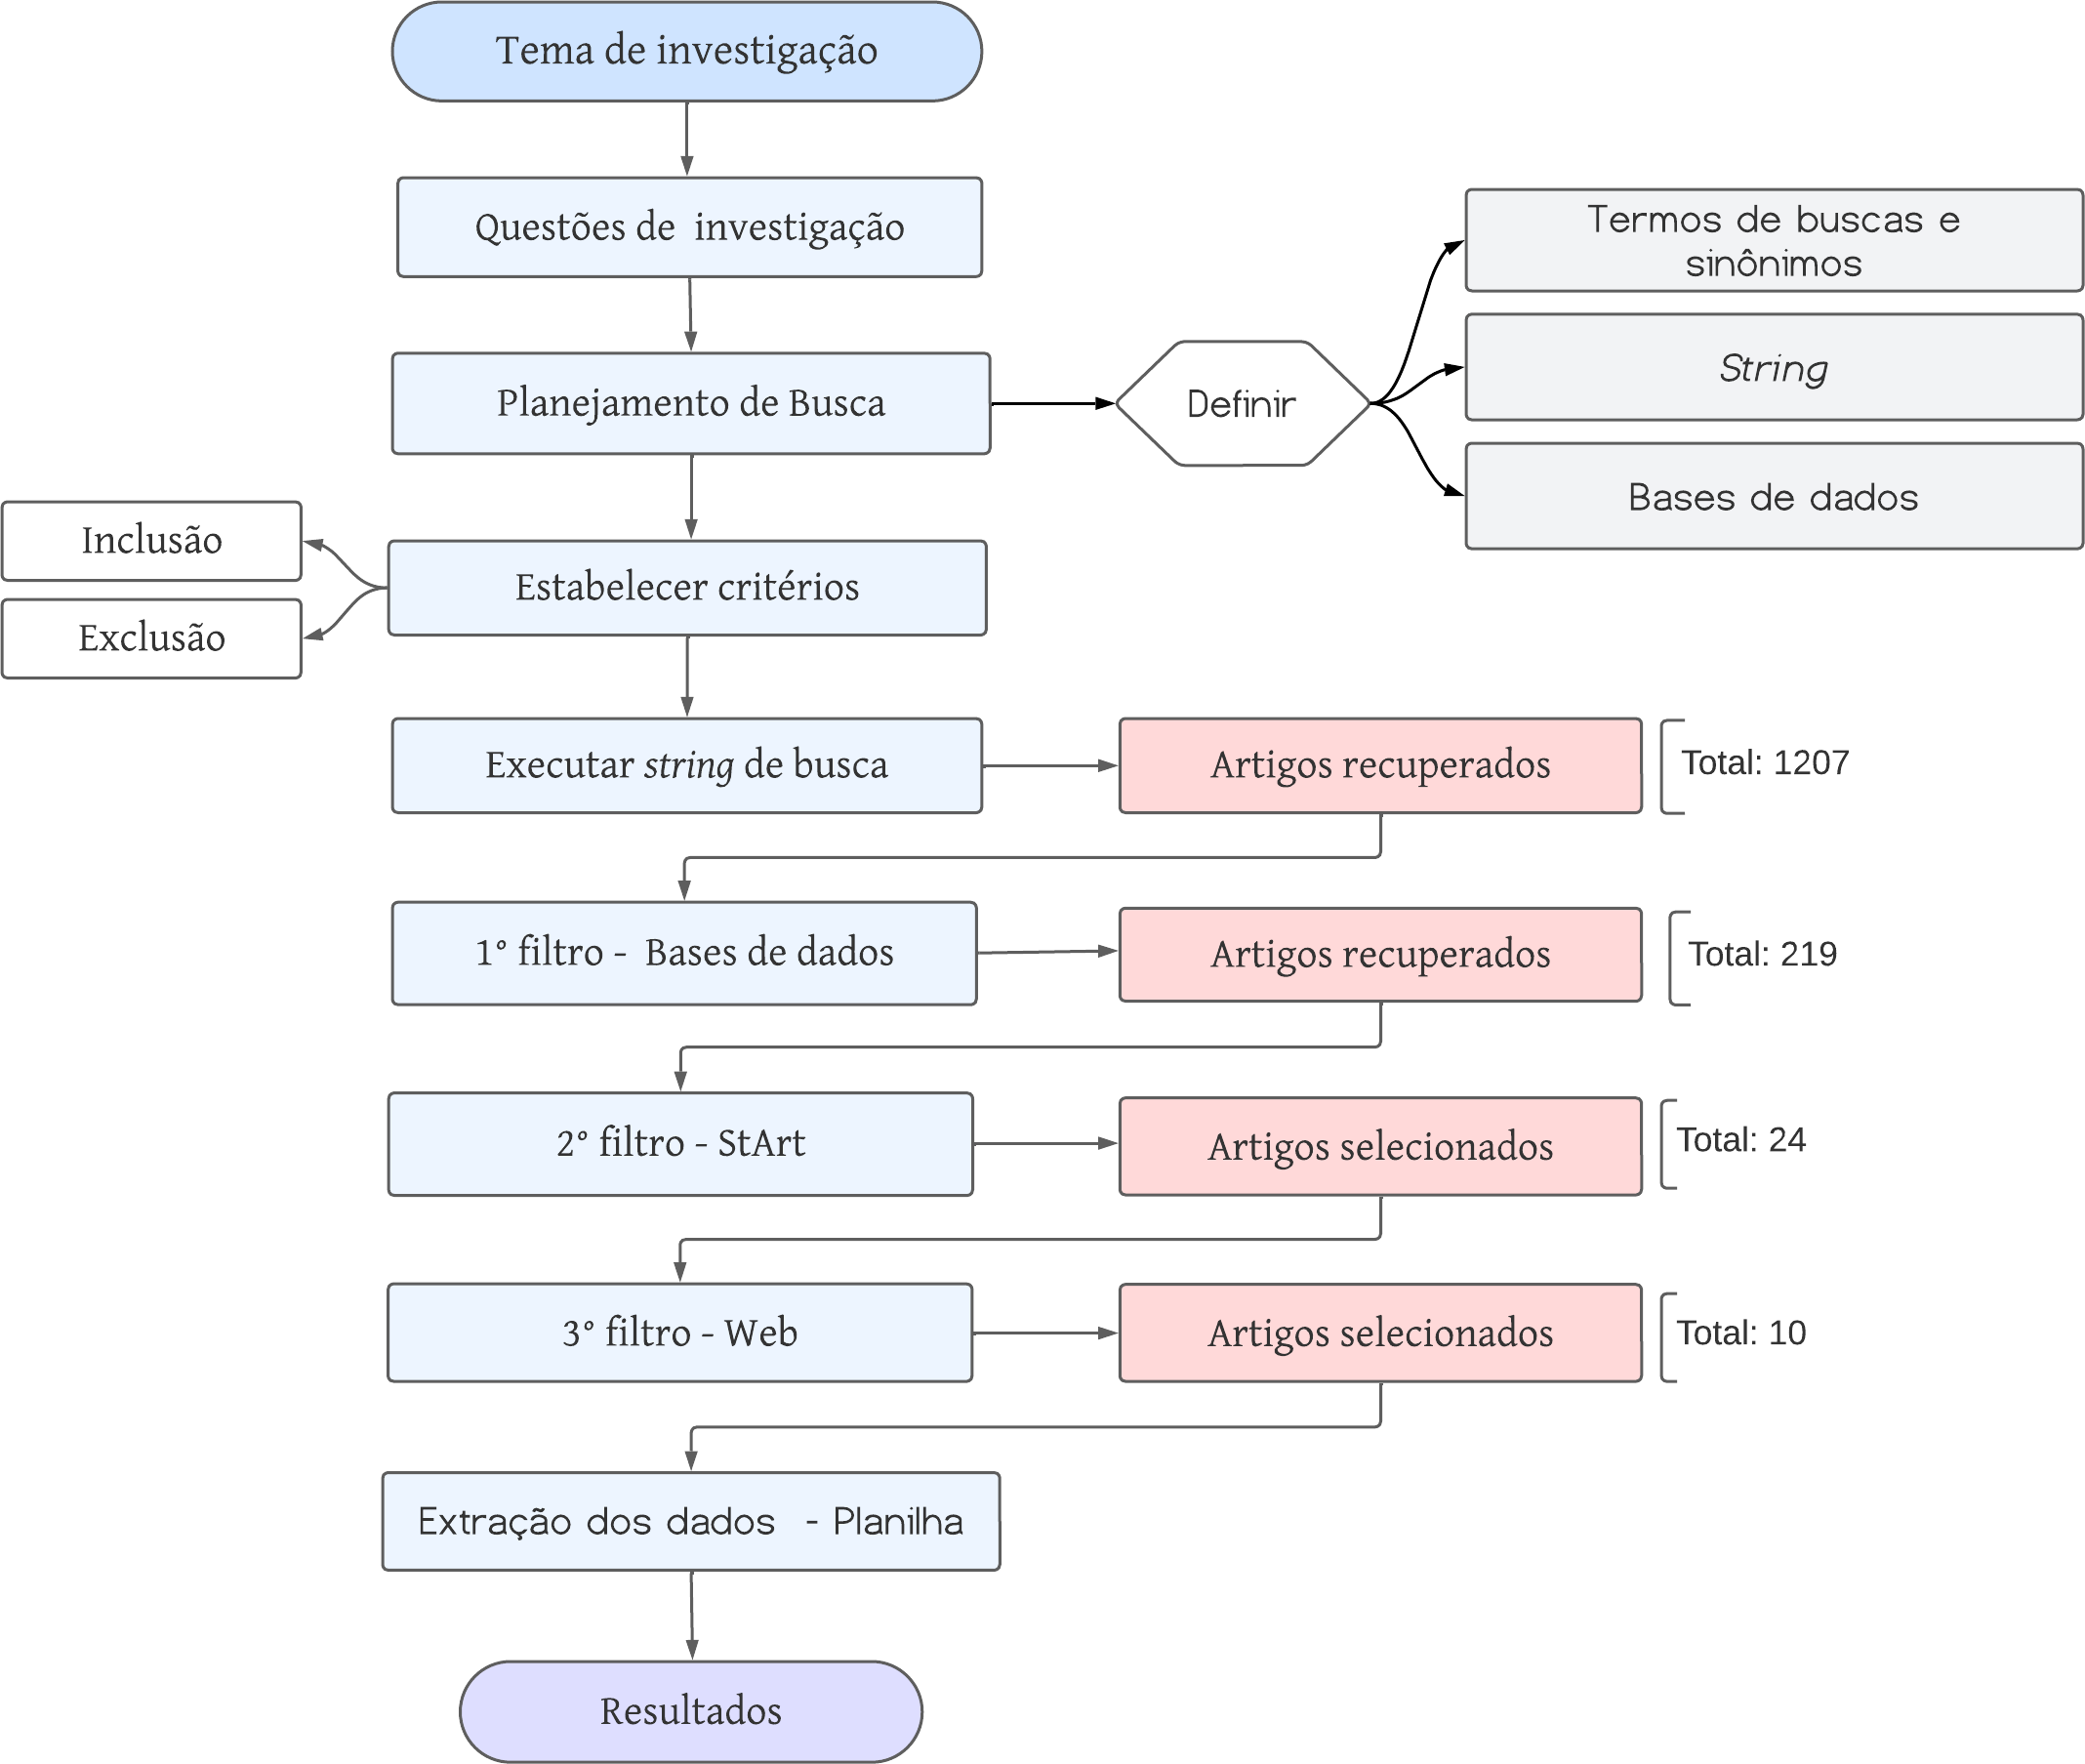
\includegraphics[width=\linewidth]{Fig1.png}
  \caption{Fluxograma da pesquisa.}
  \label{fig1}
  \source{Elaborado pelos autores.}
\end{minipage}
\end{figure}

\subsection{Definição das questões de investigação}\label{sec-fmt-manuscrito}
Para atender aos objetivos do trabalho, foi elaborada uma questão principal de pesquisa, utilizando os critérios PICO (do inglês \textit{Population}, \textit{Intervention}, \textit{Comparison} e \textit{Outcome}), e a partir dela, perguntas secundárias para viabilizar o alcance desses objetivos, bem como facilitar a compreensão e discussão dos resultados obtidos.

Assim, por população (P) pretendeu-se investigar trabalhos que trataram de “usuários de ambientes digitais”, enquanto por intervenção (I) o intuito foi investigar artigos que trouxessem coleta de dados por instrumentos, como: questionário, entrevista, observação e análise documental de registros em sistemas de informação. O critério comparação (C) não se aplica a este MSL. Como resultados (O), o objetivo foi levantar “comportamentos de risco não intencionais”. Desse modo, resultaram as seguintes questões (principal, seguida das secundárias):

\begin{enumerate}
    \item Com base em fatos registrados, observados ou autodeclarados, quais comportamentos de risco não intencionais de usuários de ambientes digitais foram identificados em trabalhos científicos?
    \item Quais grupos de usuários foram alvo de estudos sobre comportamentos de risco?
    \item Quais tipos de instrumentos de coleta de dados foram mais utilizados para investigar os comportamentos não intencionais?
    \item Quais categorias de problemas de segurança foram evidenciadas?
\end{enumerate}

\subsection{Definição dos termos de busca e sinônimos}\label{sec-formato}
A definição dos termos que fizeram parte da \textit{string} de busca considerou o objeto principal deste estudo e seu âmbito, representados pelos termos “comportamento do usuário” e “segurança da informação”, respectivamente. Considerando que o comportamento que seria investigado era o de “risco”, esse termo foi adicionado à busca. Para ampliar os resultados e minimizar o risco de perda de trabalhos relevantes na busca, foram adicionadas as traduções na língua inglesa dos termos listados, assim como sinônimos e termos relacionados.


\subsection{Definição da \textit{string} de busca}\label{sec-modelo}
Para refinamento e definição da \textit{string} de pesquisa, foram conduzidos testes de busca nas bibliotecas utilizando combinações dos termos supracitados e seus correlatos. Nesse processo, buscou-se identificar, nos títulos recuperados, correlação com o objeto de estudo deste trabalho. Além disso, como controle de eficácia da \textit{string}, foi utilizado o artigo de Santos e Silva (2021), identificado, já nas primeiras buscas, como relevante para responder às questões de pesquisa propostas. Quando se observou que a busca retornava uma quantidade significativa de títulos relacionados ao tema abordado, incluindo o artigo de controle, considerou-se que a \textit{string} estava adequadamente elaborada e alinhada ao objeto de estudo.

Desse modo, os operadores booleanos “AND” e “OR” foram utilizados para intercalar os termos de busca e seus correlatos, usando-se o primeiro para criar intersecção entre o objeto, seu atributo e o âmbito de pesquisa, enquanto o operador “OR” foi utilizado para ampliar o escopo da busca com base na união de sinônimos e termos relacionados. Esta foi a \textit{string} executada:

("cyber security" OR "cybersecurity" OR "ciberseguranca" OR "information security" OR "seguranca da informacao") AND ("human factor" OR "fator humano" OR "user behavior" OR "comportamento do usuario" OR "user habit" OR " habito do usuario") AND (risk OR risco OR ameaca OR threat OR vulnerability OR vulnerabilidade)

\subsection{Definição das bases de dados}\label{sec-organizacao}
Foram utilizadas as seguintes bases para obtenção dos artigos:
CAPES (Coordenação de Aperfeiçoamento de Pessoal de Nível Superior): atua no desenvolvimento da pós-graduação \textit{stricto sensu} do Brasil e se destaca como um dos maiores repositórios científicos virtuais do país \cite{coordenacao_de_aperfeicoamento_de_pessoal_de_nivel_superior_capes_quem_2023}.

SciELO (\textit{Scientific Electronic Library Online}) é um programa voltado para apoiar a infraestrutura de comunicação de pesquisas em acesso aberto, sendo adotado em dezesseis países que compõem a Rede SciELO, a qual reúne coleções nacionais de periódicos de qualidade \cite{scientific_electronic_library_online_scielo_programa_2023}.

Scopus, reconhecido como o maior banco de dados de resumos e citações de literatura revisada por pares, proporciona uma visão abrangente da produção global de pesquisas \cite{agencia_de_bibliotecas_digitais_da_universidade_de_sao_paulo_abd-sp_gravacao_2022}.

As bases foram selecionadas considerando sua relevância no meio acadêmico e a possibilidade de retornar dados no contexto nacional, da América Latina e mundial.

\subsection{Definição dos critérios de inclusão e exclusão}\label{sec-titulo}
Baseando-se na questão principal da pesquisa e visando descartar artigos que não tivessem relevância para respondê-la, foram estabelecidos e aplicados critérios de inclusão e exclusão, apresentados na \Cref{tab01}. Tais critérios foram executados em três etapas, analisando aspectos distintos das publicações.

O primeiro filtro foi aplicado nas bases de dados, onde ficaram estabelecidos: o recorte temporal, o idioma (português ou inglês), a disponibilidade (acesso aberto considerando a oferta gratuita na web ou a disponibilidade fornecida pela CAPES) e o tipo de material. O segundo filtro foi a leitura do título e resumo (\textit{abstract}) dos artigos, visando identificar se o artigo atendia aos critérios de inclusão. O terceiro filtro do processo de seleção se deu pela leitura completa, visando avaliar se os artigos realmente atendiam aos critérios de inclusão definidos.

\begin{table}[htbp]
\centering
\begin{threeparttable}
\caption{Critérios de inclusão e exclusão.}
\label{tab01}
\footnotesize
\begin{tabular}{*{5}{>{\raggedright\arraybackslash}p{2cm}}}
\toprule
1° Filtro - Bases & \multicolumn{2}{c}{2° Filtro - StArt} & \multicolumn{2}{c}{3° Filtro - Leitura} \\
\midrule
\textbf{Inclusão}

\textbf{CI01} – Artigos publicados entre 2018 e 2022;

\textbf{CI02} - Em português ou inglês;

\textbf{CI03} - Acesso aberto e texto integral disponível para download;

\textbf{CI04} - Ser artigo científico. &
\textbf{Inclusão}

\textbf{CI05} - Pelo título e resumo tratar de:

Fator humano;

Comportamento, hábito ou ações de risco em ambientes digitais;

\textbf{CI06} - Coletar dados de comportamento por meio dos instrumentos propostos na intervenção. &
\textbf{Exclusão}

\textbf{CE01} -  Não relaciona comportamentos de risco de usuários em ambientes digitais;

\textbf{CE02} - Artigos duplicados;

\textbf{CE03} - Não ser um artigo primário;

\textbf{CE04} - Tratar de ações intencionalmente maliciosas;

\textbf{CE05} - Tratar de um ambiente simulado. &
\textbf{Inclusão}

\textbf{CI07} - Pela leitura completa, coletar dados de comportamento de risco não intencional em ambientes digitais. &

\textbf{Exclusão}

\textbf{CE06} - Tratar apenas da conscientização do usuário;

\textbf{CE07} - Dados apresentados inviabilizam a identificação dos comportamentos objetos deste estudo. \\
\bottomrule
\end{tabular}
\source{Elaborada pelos autores.}
\end{threeparttable}
\end{table}

\subsection{Execução da \textit{string} de busca nas bases}\label{sec-autores}
A \textit{string} de busca foi executada nas bases das três bibliotecas definidas neste estudo, em 18 de outubro de 2023. O texto foi inserido integralmente em cada uma das ferramentas de busca dos sites, retornando ao todo 1207 resultados. Em seguida, para cada site foram marcados, nas caixas de seleção, os critérios de inclusão do 1° filtro, resultando em 219 artigos. A \Cref{tab02} detalha os resultados.

\begin{table}[htbp]
\centering
\begin{threeparttable}
\caption{Resultados da primeira busca.}
\label{tab02}
\begin{tabular}{l l l l}
\toprule
 Buscas & CAPES & Scopus & SciELO \\
 \midrule
Retorno da \textit{String} & 533 & 673 & 1 \\
\vspace{0.5em}\\
& Primeiro filtro \\
Recuperados por bases & 152 & 66 & 1 \\
Total & \multicolumn{3}{c}{219} \\
\bottomrule
\end{tabular}
\source{Elaborada pelos autores.}
\end{threeparttable}
\end{table}


\subsection{Baixar e armazenar o resultado das buscas}\label{sec-idioma}
As bases de dados selecionadas para este trabalho permitem exportar o conjunto de resultados obtidos nas pesquisas de busca, possibilitando seu tratamento em outro ambiente, incluindo ferramentas gerenciadoras de referências. Para auxiliar no processo de gerenciamento, utilizou-se a ferramenta ‘StArt’, que foi desenvolvida por pesquisadores da Universidade Federal de São Carlos (UFSCAR) e oferece suporte à condução de estudos secundários. Os arquivos no formato RIS foram exportados de suas bases e armazenados na aplicação StArt.

\subsection{Seleção de artigos - Segundo filtro - Análise por título e resumo (\textit{abstract})}\label{sec-resumo}
Após importar as referências para o StArt, foi iniciada a segunda aplicação dos critérios de inclusão e exclusão. Antes do tratamento pelos revisores, a ferramenta possibilita a identificação automática de trabalhos duplicados; posteriormente, permite a leitura dos títulos e resumos diretamente no ambiente da aplicação e a vinculação dos critérios pelos quais o trabalho foi rejeitado ou aceito. Seguindo esse processo, chegou-se aos seguintes resultados: 34 artigos duplicados identificados pelo StArt, 16 artigos duplicados identificados pelos pesquisadores, 145 artigos rejeitados pelos demais critérios do segundo filtro e 24 artigos selecionados para o próximo filtro.

\subsection{Seleção de artigos - Terceiro filtro - Leitura completa e Extração dos dados}\label{sec-secoes}
No terceiro filtro foi realizada a leitura integral dos 24 artigos selecionados, para se chegar a uma análise mais completa e averiguar a real relevância dos trabalhos para responder às questões de pesquisa deste MSL. Como o StArt não permite a leitura integral dentro da aplicação, optou-se por proceder esta etapa no ambiente web. Da leitura, 14 artigos não atenderam aos critérios estabelecidos desta etapa e 10 atenderam a todos os critérios, seguindo para extração. Utilizando um formulário de extração em uma planilha, foram levantadas as informações necessárias para abordar as questões de pesquisa.

\section{Resultados e discussões}\label{sec-format-simple}
Com base na extração dos artigos, realizou-se uma análise geral da disposição das evidências, apresentando características do recorte temporal, base de dados e países nos quais as pesquisas foram realizadas.

Do ponto de vista da disposição ao longo do tempo, pode-se verificar que o ano de 2021 concentra o maior número de artigos publicados, somando quatro, enquanto 2020 não teve nenhuma publicação, o que pode indicar que houve um “represamento” de artigos não concluídos no ano do ápice da pandemia de Covid-19, sendo divulgados no ano subsequente. A \Cref{fig2} ilustra os quantitativos de artigos nos cinco anos do recorte.

\begin{figure}[htbp]
\centering
\begin{minipage}{0.65\linewidth}
  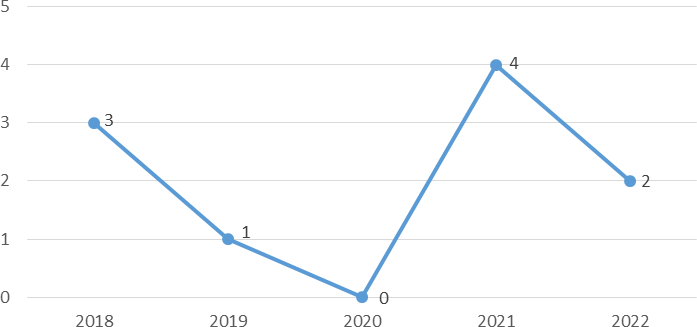
\includegraphics[width=\linewidth]{Fig2.png}
  \caption{Artigos publicados por ano.}
  \label{fig2}
  \source{Elaborado pelos autores.}
\end{minipage}
\end{figure}

Das três bibliotecas pesquisadas, a Capes teve mais conteúdo que respondeu positivamente aos critérios de inclusão propostos, seguida de Scopus e SciELO, conforme \Cref{fig3}.

\begin{figure}[htbp]
\centering
\begin{minipage}{0.65\linewidth}
  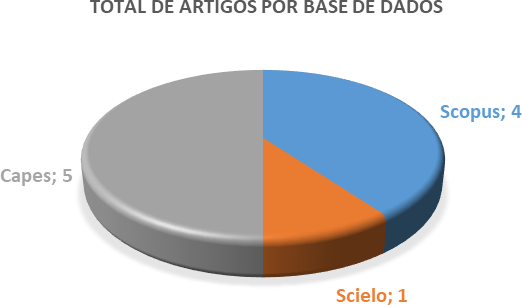
\includegraphics[width=\linewidth]{Fig3.png}
  \caption{Artigos publicados por base de dados.}
  \label{fig3}
  \source{Elaborado pelos autores.}
\end{minipage}
\end{figure}

Considerando a análise da distribuição geográfica dos países nos quais a coleta de dados foi aplicada, observa-se que ela abrangeu pelo menos seis nações. As maiores contribuições foram da Arábia Saudita e Polônia, cada uma totalizando dois artigos. O Brasil, por sua vez, teve representação em apenas um artigo. A \Cref{tab03} resume essa distribuição geográfica, destacando o número de artigos provenientes de cada país:

\begin{table}[htbp]
\centering
\begin{threeparttable}
\caption{Distribuição geográfica.}
\label{tab03}
\begin{tabular}{ll}
\toprule
País & Quantidade \\
\midrule
Arábia Saudita & 2 \\
Polônia & 2 \\
Não especificado & 2 \\
Brasil & 1 \\
Croácia & 1 \\
Inglaterra & 1 \\
Romênia & 1 \\
\midrule
\end{tabular}
\source{Elaborado pelos autores.}
\end{threeparttable}
\end{table}

A partir deste ponto, serão detalhados os resultados extraídos dos artigos que abordaram as questões de investigação propostas neste estudo, conforme descrito na metodologia (Seção \ref{sec-fmt-manuscrito}). Essa análise contribui para uma visão mais abrangente e informada sobre o tema em questão.

\textbf{Q1.} Com base em fatos registrados, observados ou autodeclarados, quais comportamentos de risco não intencionais de usuários de ambientes digitais foram identificados em trabalhos científicos?

Para discutir essa questão, identificou-se a partir dos artigos os comportamentos de risco mais significativos destacados pelos autores. No entanto, no Apêndice \ref{apx-longtable} estão listados todos os comportamentos mapeados neste trabalho.

\textcite{rindasu_information_2018}, utilizando o método de coleta de dados por meio de um questionário com 49 estudantes do programa de Mestrado em Contabilidade, Auditoria e Sistemas de Informação de Gestão de uma universidade na Romênia, em que teve como objetivo analisar a percepção dos participantes em relação à segurança de dados nos campos financeiros e contábeis, constatou que 63\% dos entrevistados mantém senhas anotadas no local de trabalho, 41\% não verifica anexos de \textit{e-mail} de remetentes conhecidos e 55\% não verifica de conhecidos ou desconhecidos.

No estudo conduzido por \textcite{palega_threats_2018} acerca dos comportamentos dos funcionários em uma empresa de construção na Polônia, embora não tenham sido fornecidos detalhes sobre o número de participantes, os resultados destacam que mais de 63\% dos envolvidos utilizaram o \textit{e-mail} corporativo para atividades pessoais. Além disso, observou-se que até 80\% usaram o \textit{hardware} da empresa para propósitos não vinculados às responsabilidades oficiais.

\textcite{galba_evidential_2018} conduziram uma pesquisa envolvendo 627 usuários de \textit{e-mail}. Apesar de não terem especificado a região geográfica, o objetivo do estudo era analisar o comportamento desses usuários. Na análise detalhada das respostas, os pesquisadores concluíram que esses usuários raramente diferenciam a comunicação privada da profissional. A maioria utiliza serviços de \textit{e-mail} gratuitos, como Gmail e Yahoo, para fins profissionais, e raramente emprega um terceiro endereço de \textit{e-mail} “temporário” para registros em serviços online questionáveis. Além disso, observaram que frequentemente os usuários utilizam computadores públicos com proteção de \textit{software} questionável para acessar o sistema de \textit{e-mail} e que raramente consideram a proteção de \textit{software} em seus computadores pessoais.

Na Croácia, \textcite{erceg_information_2019} investigou o comportamento em segurança da informação entre profissionais de saúde (88 participantes) e colaboradores de uma empresa privada (64 participantes), totalizando 152 entrevistados. O estudo utilizou um questionário abrangendo comportamento, conhecimento e consciência do usuário. O autor destacou que 9,9\% dos participantes admitiram fornecer seus dados oficiais de acesso, como nome de usuário e senha, a colegas de trabalho. Além disso, 32\% nunca utilizam mais de um endereço de \textit{e-mail} (um para uso privado e outro para uso oficial), e 63,8\% não bloqueiam o computador durante breves ausências do local de trabalho.

\textcite{alsharif_impact_2022} investigaram vulnerabilidades humanas em senhas, redes sociais, engenharia social e \textit{phishing}, na Arábia Saudita, com 333 participantes (sendo 74\% homens e 26\% mulheres) por meio de questionários. Os resultados indicaram que 78\% dos participantes não alteram frequentemente suas senhas, 74\% usam informações pessoais, como aniversário, nome do pai ou do filho em suas senhas, e 64\% utilizam ou ocasionalmente utilizam dados precisos em aplicativos sociais, como "aniversário, cidade". Além disso, 71\% não empregam anti-spam e 41\% não adotam autenticação de dois fatores ao desbloquear dispositivos ou programas.

\textcite{mohammed_locked_2021}, na Inglaterra, conduziram um estudo observacional nas áreas clínicas (enfermarias) acessíveis aos pacientes em um Hospital Geral Regional, com o objetivo de verificar se os computadores desocupados estavam bloqueados. Os resultados revelaram que dos 58 computadores observados, 36 estavam desocupados, dentre os quais 18 estavam desbloqueados, ou seja, 50\% da amostra dos computadores desocupados estavam sem bloqueio.

\textcite{antunes_integrated_2021}, embora não tenham especificado a região geográfica de onde ocorreu a pesquisa, realizaram um estudo com estudantes do 6º e 9º anos, utilizando questionário com Escala Likert de 1 a 7 para avaliar atitudes e comportamentos em segurança cibernética. Os resultados evidenciaram comportamentos negativos em algumas áreas. No tocante ao armazenamento de informações, apenas 64\% dos estudantes apresentaram comportamento positivo, apontando que uma parcela significativa (36\%) não adota práticas seguras nesse aspecto. Quando questionados sobre o comportamento ao serem contatados por estranhos, somente 46\% afirmaram que clicam apenas em links vindos de pessoas de confiança. Em relação à verificação de atualizações para programas antivírus, os alunos também demonstraram um comportamento negativo significativo, com 62\% apresentando atitudes negativas nesse aspecto.

\textcite{santos_gestao_2021} buscaram identificar os comportamentos inseguros praticados em uma Instituição da Administração Pública Federal Brasileira, assim como os possíveis fatores a eles associados. Para tal, realizaram coleta em duas etapas. Num primeiro momento, foi utilizada a ferramenta de registro de ordens de serviço da Central de Serviços, o programa de inventários de \textit{hardware} e \textit{software} computacional, relatórios do servidor de antivírus e entrevistas semiestruturadas com funcionários do Departamento de TI para identificar ocorrências geradas por comportamentos irregulares relacionados à segurança da informação, dos 15 meses anteriores à pesquisa. Então, constataram que houve um número significativo de ocorrências geradas por comportamentos de riscos, como: compartilhamento de senhas, antivírus removidos, \textit{softwares} instalados sem licença, alterações da configuração padrão do sistema operacional, aplicações em produção desenvolvidas por funcionários não autorizados e compartilhamentos de diretórios permitindo o acesso a dados sensíveis.

No segundo momento, foram descritos comportamentos inseguros coletados por meio da observação direta da atividade de trabalho de oito pessoas, durante uma hora de trabalho. Dentre os comportamentos observados, todos os provenientes da etapa anterior se repetiram, com exceção de alterações da configuração padrão do sistema operacional. Ainda puderam ser apontados outros comportamentos, dos quais podem ser destacados: não bloqueio da tela ao se ausentar, armazenamento de dados corporativos em mídias do tipo \textit{flash memory} e utilização de \textit{notebook} pessoal na rede local.

\textcite{szczepaniuk_analysis_2022} focaram seu estudo em 1520 participantes do setor empresarial da Polônia. O questionário abordou segurança técnica e medidas de proteção de dados no ciberespaço, usando uma escala Likert para avaliar atitudes e comportamentos. Os resultados indicaram que a maioria dos participantes se envolve em atividades potencialmente perigosas no ciberespaço, com percentuais consideráveis em práticas arriscadas: \textit{download} de \textit{software} ilegal (84\%), uso de sites potencialmente perigosos (71\%), uso de Wi-Fi público (67\%) e abertura de anexos e links de fontes desconhecidas (59\%). Os estudos revelaram ainda que 21\% dos respondentes nunca verificam mídia externa de armazenamento, 20\% não usa autenticação de dois fatores e 18\% não verifica anexos em \textit{e-mails} recebidos.

\textcite{alissa_appling_2022}, através de um questionário gamificado, buscou rastrear e examinar o comportamento do usuário por meio de perguntas relacionadas a senha, identidade, \textit{e-mail}, dados confidenciais e segurança física na Arábia Saudita. O estudo envolveu 48 participantes, e ao término do jogo, o relatório estatístico apresentado pelos autores revelou que, em relação a senhas, \textit{e-mails} e dados confidenciais, 67\% dos participantes utilizavam senhas simples e 40\% compartilhavam sua senha.

\textbf{Q2.} Quais grupos de usuários foram alvo de estudos sobre comportamentos de risco?

Diferentes grupos de usuários foram alvo de estudos sobre comportamentos de risco, conforme demonstrado na \Cref{fig4}. A análise detalhada revelou uma variedade de segmentos, incluindo estudantes de nível fundamental e mestrado, profissionais da saúde, funcionários públicos e privados, usuários de \textit{e-mail} e a população em geral. Isso aponta a universalidade dos problemas de segurança digital e a importância de conscientização em diferentes contextos.

\begin{figure}[htbp]
\centering
\begin{minipage}{0.85\linewidth}
  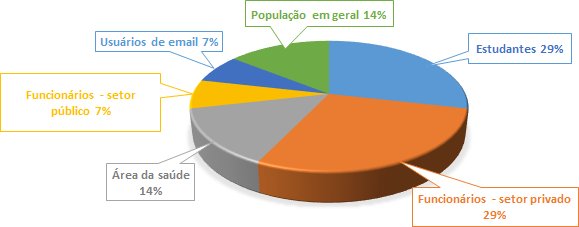
\includegraphics[width=\linewidth]{Fig4.png}
  \caption{Grupo de usuários.}
  \label{fig4}
  \source{Elaborado pelos autores.}
\end{minipage}
\end{figure}

\textbf{Q3.} Quais tipos de instrumentos de coleta de dados foram mais utilizados para investigar os comportamentos não intencionais?

Dentre os instrumentos de coleta de dados empregados, destaca-se o questionário como o mais frequente, totalizando sete ocorrências. Além disso, a observação global foi empregada em dois estudos, sendo que em um deles foi combinada com uma análise documental e entrevistas semiestruturadas. Vale ressaltar também o uso singular de um questionário gamificado, indicando uma abordagem inovadora na coleta de informações sobre comportamentos de segurança (\Cref{fig5}).

Essa diversidade de métodos de coleta de dados reflete a abordagem multifacetada adotada para compreender e analisar os comportamentos não intencionais em contextos específicos.

\begin{figure}[htbp]
\centering
\begin{minipage}{0.85\linewidth}
  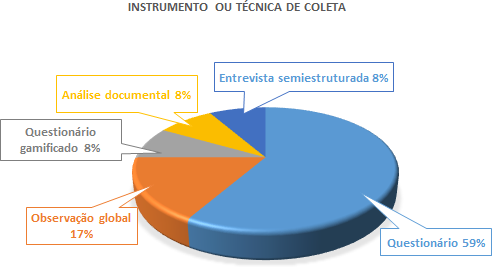
\includegraphics[width=\linewidth]{Fig5.png}
  \caption{Instrumento ou técnica de coleta.}
  \label{fig5}
  \source{Elaborado pelos autores.}
\end{minipage}
\end{figure}

\textbf{Q4.} Quais categorias de problemas de segurança foram evidenciadas?
Os autores deste MSL identificaram um total de 97 quesitos investigativos sobre comportamentos incidentais que foram objeto de pesquisa. Esses quesitos foram agrupados por semelhança em dez aspectos da segurança, com o objetivo de categorizar os principais temas investigados, como pode ser observado na \Cref{fig6}.

\begin{figure}[htbp]
\centering
\begin{minipage}{0.85\linewidth}
  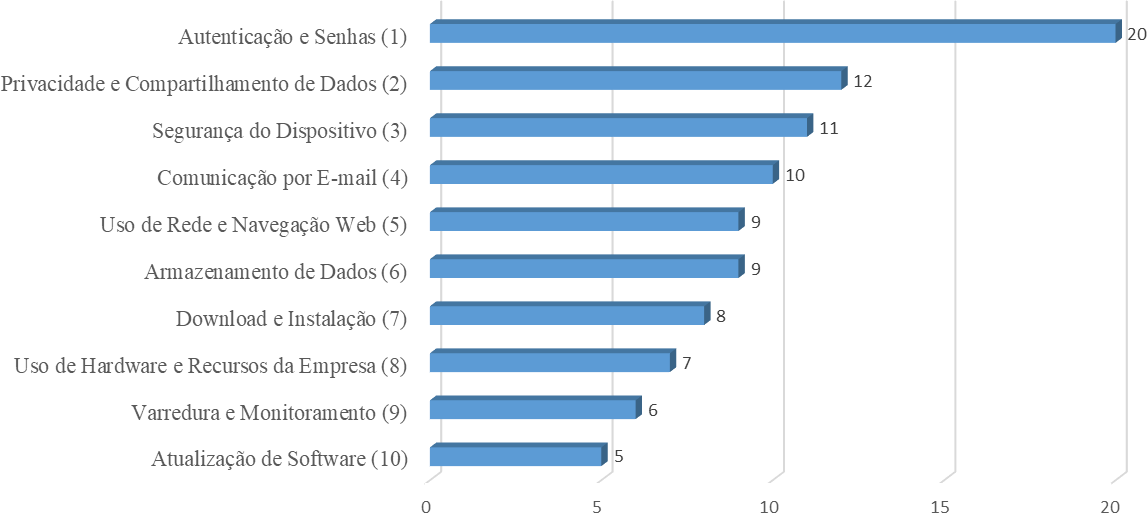
\includegraphics[width=\linewidth]{Fig6.png}
  \caption{Categorização dos quesitos investigados.}
  \label{fig6}
  \source{Elaborado pelos autores.}
\end{minipage}
\end{figure}

Dentre as categorias, destacam-se: ‘Autenticação e Senhas’, com 20 quesitos relacionados a esse tema; ‘Privacidade e Compartilhamento de Dados’, com 12 quesitos; ‘Segurança do Dispositivo’, com 11 quesitos; e ‘Comunicação por E-mail’, com 10 quesitos. Juntas, essas categorias representam mais da metade do total de quesitos.
 
Em relação à quantidade de artigos que tratam dessas categorias, observa-se que ‘Autenticação e Senhas’ é abordada em 7 artigos, enquanto ‘Segurança do Dispositivo’ aparece em 6 artigos. Por sua vez, ‘Comunicação por E-mail’ é discutida em 5 artigos, e ‘Privacidade e Compartilhamento de Dados’ é mencionada em 4 artigos (\Cref{fig7}).

\begin{figure}[htbp]
\centering
\begin{minipage}{0.85\linewidth}
  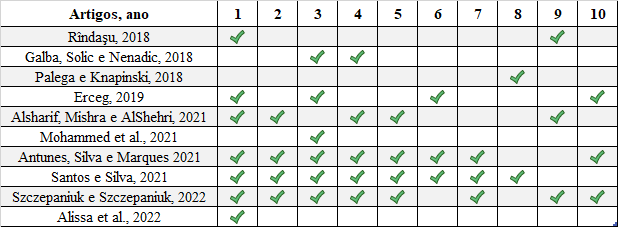
\includegraphics[width=\linewidth]{Fig7.png}
  \caption{Categorias abordadas por artigos.}
  \label{fig7}
  \source{Elaborado pelos autores.}
\end{minipage}
\end{figure}

Esses números indicam que essas quatro áreas foram mais frequentemente investigadas no contexto de comportamentos não intencionais em segurança da informação. No entanto, apesar de as demais áreas não estarem significativamente distantes das primeiras em termos de atenção, ainda há espaço para aprofundar investigações e pesquisas relacionadas a elas. Compreender de forma holística o comportamento dos usuários é fundamental para desenvolver políticas de conscientização mais eficazes.

\section{Conclusão}\label{sec-links}
A crescente dependência de dispositivos digitais e a frequente interação com tecnologias destacam a necessidade de compreender e mitigar os riscos oriundos das ações inadvertidas dos usuários. Por isso, o presente artigo identificou, por meio de um mapeamento sistemático de literatura, evidências de comportamentos não intencionais dos usuários de ambientes digitais. O estudo revelou um cenário diversificado ao evidenciar uma série de práticas de risco que permeiam as interações cotidianas, como compartilhamento de senhas, remoção de antivírus e abertura de links de remetentes desconhecidos, expondo vulnerabilidades significativas nos sistemas de segurança da informação.

Ficou demonstrado que diferentes grupos de usuários, desde estudantes até profissionais de diversas áreas, foram alvo de estudos que investigaram esses comportamentos de risco. Essa diversidade de públicos reflete a amplitude do desafio enfrentado na promoção da conscientização e na implementação de medidas eficazes de segurança digital.

Os instrumentos de coleta de dados, principalmente questionário e observação, desempenharam um importante papel na identificação e análise desses comportamentos, proporcionando uma compreensão abrangente das práticas arriscadas adotadas pelos usuários. Além disso, as categorias de problemas de segurança mais evidenciadas, como ‘Autenticação e Senhas’, ‘Privacidade e Compartilhamento de Dados’, ‘Segurança do Dispositivo’ e ‘Comunicação por E-mail’ apontam para áreas que estiveram no foco da atenção dos trabalhos, enquanto as outras áreas estudadas ainda demandam melhor investigação para compreensão e desenvolvimento de estratégias mais eficazes de proteção cibernética.

Uma limitação identificada neste estudo diz respeito à possível vantagem que poderia ter sido alcançada com a inclusão de um maior número de bases de dados, visando enriquecer a pesquisa e proporcionar uma amostra de artigos mais abrangente e representativa, especialmente no tocante a artigos brasileiros, visto que apenas um artigo nacional integrou os resultados desta pesquisa. Adicionalmente, enfrentou-se dificuldades na interpretação de alguns artigos e com a falta de acesso a bibliotecas especializadas em Tecnologia da Informação, cujo conteúdo estava sujeito a custo.

Este estudo visa subsidiar iniciativas e pesquisas voltadas a aprimorar a conscientização e os hábitos no ambiente digital, especialmente no que diz respeito a comportamentos incidentais. Além disso, busca contribuir para a criação de políticas e práticas de segurança da informação mais eficazes. Por fim, espera-se que este artigo incite uma reflexão nos leitores acerca de seus hábitos relacionados à segurança de dados e à navegação no ambiente virtual.

Para futuras pesquisas, sugere-se a realização de uma pesquisa empírica que aborde a temática deste trabalho, para compreender o nível de conscientização e os fatores que influenciam tais comportamentos. Subsequentemente, sugere-se a criação de um material educativo, como uma cartilha de boas práticas, que explore propostas facilmente aplicáveis no cotidiano, transcendendo a visão convencional da política de segurança como norma e incentivando a aprendizagem e a adoção contínua de comportamentos seguros. Atualmente, no CGI.br, existem cartilhas disponíveis para consulta como a Cartilha de Acessibilidade na Web, o Guia de Boas Práticas para Acessibilidade Digital, o Guia Internet Segura para seus filhos (2ª edição), entre outros materiais que auxiliam como material educativo. Porém, seria interessante o desenvolvimento de cartilhas que explorassem os comportamentos de risco no ambiente digital.

%Adicionar Apêndice com quadros

\printbibliography\label{sec-bib}
%conceptualization,datacuration,formalanalysis,funding,investigation,methodology,projadm,resources,software,supervision,validation,visualization,writing,review
\begin{contributors}[sec-contributors]
\authorcontribution{Ângela Rayne Nogueira Alves}[conceptualization,datacuration,formalanalysis,methodology,investigation]
\authorcontribution{Jean Marcel Hora Alves}[conceptualization,datacuration,formalanalysis,methodology,investigation]
\authorcontribution{Igor Oliveira Vasconcelos}[projadm]
\authorcontribution{Cleide Ane Barbosa da Cruz}[projadm]
\end{contributors}

\appendix
\section{APÊNDICE A – Comportamento identificado}\label{apx-longtable}

Os quadros A1 a A4 apresentam uma compilação de todos os comportamentos identificados nos estudos selecionados. Cada linha representa um comportamento específico, indicando quem conduziu o estudo (autor), o ano em que foi publicado e a frequência de ocorrência na amostra.

%\setcounter{table}{0}
%\renewcommand{\tablename}{Quadro}
%renewcommand{\thetable}{A\arabic{table}}
\begin{footnotesize}
\begin{longtable}{p{2cm} p{5cm} p{3cm}}
\caption{Comportamento identificado em 2018.}
\label{tab01-appendix}
\\
\toprule
Autor, ano & Comportamento identificado & Frequência \\
\midrule
Galba, Solic e Nenadic, 2018 & Não distinguir entre comunicações de \textit{e-mail} pessoais e profissionais & Frequentemente \\
& Utilizar serviços de \textit{e-mail} gratuitos para comunicação profissional & Frequentemente \\
& Utilizar endereço de \textit{e-mail} pessoal ou profissional para se registrar em serviços da Internet considerados questionáveis em termos de segurança & Frequentemente \\
& Utilizar PCs públicos com proteção de software questionável para acessar o sistema de \textit{e-mail} & Frequentemente \\
& Desconsiderar a proteção de software em PCs pessoais & Frequentemente \\
\midrule
Rîndaşu et al., 2018 & Manter senhas anotadas no local de trabalho & 63\% \\
& Não verificar os anexos de \textit{e-mails} de remetentes conhecidos ou desconhecidos & 55\% \\
& Não verificar os anexos de \textit{e-mails} de remetentes conhecidos & 41\% \\
\midrule
Palega e Knapinski, 2018 & Utilizar o hardware informático da empresa para: & \\
& Navegar na web & 80\% \\
& Visualizar \textit{e-mails} pessoais & 63\% \\
& Utilizar mensageiros instantâneos & 26\% \\
& Utilizar de redes sociais & 23\% \\
& Jogar jogos de computador & 9\% \\
& Instalar vários tipos de \textit{software} e aplicativos & 9\% \\
\bottomrule
\source{Elaborada pelos autores.}
\end{longtable}
\end{footnotesize}


\begin{footnotesize}
\begin{longtable}{p{2cm} p{5cm} p{3cm}}
\caption{Comportamento identificado em 2019.}
\label{tab02-appendix}
\\
\toprule
Autor, ano & Comportamento identificado & Frequência \\
\midrule
Erceg, 2019 & Bloquear o computador de trabalho ao sair	por um curto período de tempo & 77\% Raramente ou nunca \\
& Compartilhar senha de acesso ao próprio e-mail & 65,3\% Eu e pelo
menos mais uma pessoa \\
& Atualizar outros programas e o sistema operacional do seu computador & 64\% Raramente ou nunca \\
& Compartilhar senha de acesso ao e-mail corporativo & 60,9\% Eu e pelo menos mais uma pessoa \\
& Manter a proteção do computador & 54\% Raramente ou nunca \\
& Última vez que fez um \emph{backup} de arquivos e documentos pessoais
& 51,9\% Nunca ou não lembra \\
& Usar senhas diferentes para sistemas diferentes & 47\% Raramente ou nunca \\
& Fazer \emph{logoff} depois de terminar o trabalho & 18\% Raramente ou nunca \\
& Compartilhar dados oficiais de acesso a colegas de trabalho & 14\% Às vezes, frequentemente ou sempre \\
\bottomrule
\source{Elaborada pelos autores.}
\end{longtable}
\end{footnotesize}


\begin{footnotesize}
\begin{longtable}{p{2cm} p{5cm} p{3cm}}
\caption{Comportamento identificado em 2021.}
\label{tab03-appendix}
\\
\toprule
Autor, ano & Comportamento identificado & Frequência \\
\midrule
Alsharif, Mishra e AlShehri, 2021 & Alterar	senha com frequência & 78\% Não ou às vezes \\
& Usar informações pessoais na senha. Ex.: ``aniversário, nome do pai, nome do filho'' & 74\% Sim \\
& Usar anti-spam & 71\% Não \\
& Usar informações precisas em aplicativos sociais. Ex.: ``seu aniversário, cidade'' & 64\% Sim ou às vezes \\
& Fazer logout do seu e-mail depois de terminar de usar & 62\% Não ou às vezes \\
& Compartilhar informações com outras pessoas por meio de aplicativos de redes sociais & 48\% Sim ou às vezes \\
& Abrir qualquer e-mail que chega à sua caixa de entrada & 41\% Sim ou às vezes \\
& Utilizar autenticação de dois fatores ao desbloquear o dispositivo ou os programas & 41\% Não \\
& Utilizar senhas simples & 37\% Simples \\
& Utilizar senha diferente para suas contas & 30\% Não \\
& Usar sites desconhecidos para comprar & 22\% Sim ou talvez \\
\midrule
Mohammed \emph{et al}., 2021 & Não bloquear o computador ao se ausentar da estação de trabalho & 50\% \\
\midrule
Antunes, Silva e Marques, 2021 & Verificar	atualizações de qualquer \emph{software} antivírus que você tenha instalado & 62\% \\
& Clicar em links em uma mensagem de e-mail proveniente de um amigo ou colega de confiança & 54\% \\
& Verificar se o \emph{software} em seu smartphone/tablet/laptop/PC está atualizado & 43\% \\
& Usar a mesma senha para vários sites & 41\% \\
& Armazenar informações pessoais, de família e amigos em seu dispositivo	eletrônico pessoal (por exemplo, smartphone/tablet/laptop) & 36\% \\
& Usar Wi-Fi público de acesso gratuito & 32\% \\
& Usar sistemas de armazenamento online para trocar e manter informações pessoais ou sensíveis & 21\% \\
& Aceitar solicitações de amizade nas redes sociais porque reconhece a foto & 21\% \\
& Baixar mídia digital (músicas, filmes, jogos) de fontes não licenciadas & 18\% \\
& Compartilhar minha localização atual nas redes sociais & 9\% \\
& Baixar dados e materiais de sites no seu computador sem verificar sua	autenticidade & 9\% \\
& Usar senhas simples & 7\% \\
& Transferir dados da escola para mídia flash própria & 7\% \\
& Baixar \emph{software}/aplicativos antivírus gratuitos de uma fonte desconhecida & 4\% \\
& Desativar o antivírus do meu computador para poder baixar informações	de sites & 3\% \\
& Inserir informações de pagamento em sites que não possuem informações/certificações claras de segurança & 1\% \\
& Compartilhar senhas & 0\% \\
& Clicar em links contidos em e-mails não solicitados de uma fonte desconhecida & 0\% \\
& Enviar informações pessoais para pessoas desconhecidas pela Internet & 0\% \\
\midrule
Santos e Silva, 2021 & Compartilhar senhas & 88\% \\
& Não bloquear a tela ao se ausentar & 75\% \\
& Armazenar dados corporativos em mídias do tipo flash memory & 38\% \\
& Fazer \emph{backup} em mídias do tipo ópticas & 38\% \\
& Utilizar notebook pessoal na rede local & 38\% \\
& Armazenar arquivos em diretórios públicos nas estações de trabalho & 25\% \\
& Armazenar dados corporativos na estação de trabalho & 25\% \\
& Desenvolvimento de sistemas de informação por funcionários não autorizados & 25\% \\
& Utilizar e-mail pessoal para assuntos institucionais & 25\% \\
& Armazenar dados pessoais no driver de rede & 13\% \\
& Compartilhar permissões além das necessárias & 13\% \\
& Instalar programas não autorizados & 13\% \\
& Remover antivírus & 13\% \\
& Rotina inadequada de \emph{backup} & 13\% \\
& Trocar senha periodicamente & 13\% \\
& Comportamento identificado por análise documental: \\
& Remover \emph{software} antivírus & 5 ocorrências \\
& Instalar suíte de escritório sem licença & 97 ocorrências \\
& Alterar a configuração padrão do sistema operacional & 2 ocorrências \\
& Instalação de \emph{software} desenvolvido por funcionário não autorizado & 15 ocorrências \\
& Compartilhar diretório permitindo o acesso a dados sensíveis & 7 ocorrências \\
& Compartilhar senhas & 1 ocorrência \\
\bottomrule	
\source{Elaborada pelos autores.}
\end{longtable}
\end{footnotesize}


\begin{footnotesize}
\begin{longtable}{p{2cm} p{5cm} p{3cm}}
\caption{Comportamento identificado em 2022.}
\label{tab04-appendix}
\\
\toprule
Autor, ano & Comportamento identificado & Frequência \\
\midrule
Szczepaniuk e Szczepaniuk, 2022 & Anonimização do tráfego web & 86\% às vezes, raramente ou nunca \\
& Verificar anexos de e-mail com \emph{software} antivírus & 84\% às vezes, raramente ou nunca \\
& Verificar o computador em busca de \emph{malware} & 84\% às vezes, raramente ou nunca \\
& Baixar \emph{software} ilegal & 84\% às vezes, frequentemente ou sempre \\
& Usar navegadores web que não armazenam o histórico de buscas & 83\% às vezes, raramente ou nunca \\
& Usar autenticação de dois fatores & 80\% às vezes, raramente ou nunca \\
& Verificar mídia de armazenamento externo & 74\% às vezes, raramente ou nunca \\
& Alterar senha regularmente e aplicar senhas de complexidade adequada & 73\% às vezes, raramente ou nunca \\
& Permitir que terceiros acessem e usem dados pessoais & 73\% às vezes, raramente ou nunca \\
& Ler políticas de privacidade e termos de uso de sites & 72\% às vezes, raramente ou nunca \\
& Consentir o perfil de dados & 72\% às vezes, frequentemente ou sempre \\
& Desativar serviços de geolocalização em um sistema operacional & 71\% às vezes, raramente ou nunca \\
& Utilizar sites potencialmente inseguros & 71\% às vezes, frequentemente ou sempre \\
& Utilizar redes Wi-Fi públicas & 67\% às vezes, frequentemente ou sempre \\
& Utilizar sites com protocolo HTTPS & 61\% às vezes, raramente ou nunca \\
& Abrir anexos e links de fontes desconhecidas & 59\% às vezes, frequentemente ou sempre \\
& Atualizar base de dados de vírus em \emph{software} antivírus & 58\% às vezes, raramente ou nunca \\
& Atualizar \emph{software} (incluindo sistema operacional) & 56\% às vezes, raramente ou nunca \\
& Visualizar spam e outras mensagens de fontes desconhecidas & 53\% às vezes, frequentemente ou sempre \\
& Ajustar configurações padrão de privacidade em redes sociais conforme as necessidades individuais & 50\% às vezes, raramente ou nunca \\
\midrule
Alissa \emph{et al}., 2022 & Usar senhas simples & 67\% usam \\
& Compartilhar senhas & 40\% compartilham \\
\bottomrule	
\source{Elaborada pelos autores.}
\end{longtable}
\end{footnotesize}

		

\end{document}


